\chapter{実装}
\label{chap:implementation}

% \section{めも}

% Linuxカーネルのバージョン,System.mapの情報およびconfigの情報を知らなければ,メモリのみから正しくコンテキストを復元していくことはできない.

% libtlpの論文(もうちょっとちゃんと書く)で紹介されているprocess-list.cはSystem.mapを引数として渡し,
% init\_taskの行をreadすることでinit\_taskの仮想アドレスを得ている.
% また,カーネルコンフィグに依存するマクロの値や,使用する関数などもハードコーディングされており,論文の環境以外で動かすことが容易ではない.

\section{実装の概要}

本研究では,RDMAを用いて,動作中のマシンのメモリの値を取得していくことで,リモートホストから監視対象ホストのオペレーティングシステムのコンテキストを復元していくことを目指す.
この目的を実現するために,本研究では,NetTLP\cite{246316}を用いて実験を行う.

\section{NetTLP}
\label{section:nettlp}

NetTLPの目的は,PCIeデバイスの開発プラットフォームである.

その機能の一つとして,DMA messageとethernetパケットを相互変換する機能がある.
\ref{chap:related_works}章で述べたが,RDMAのInfiniband実装は,制限が多い.
% (もう少し詳しく(3章に詳しく書く))
NetTLPにおけるRDMAでは,物理アドレスを指定することで,1Byteから4096Byteまでの任意のバイト数の値を取得することが可能である.
また,NetTLPを用いたRDMAでは,メインメモリの全メモリアドレスにアクセスすることが可能であり,アクセスできないメモリアドレスは存在しない,
すなわち全メモリアドレス空間から値を取得することが可能となっている.

NetTLPはFPGAボード上で動作するものであり,これを利用するためのインターフェースとして,libtlpが用意されている.
libtlpでは,RDMAを用いてメモリダンプを取得するためのインターフェースが関数として用意されている.
この関数を含んだヘッダファイルをincludeし,プログラムから呼び出すことで,メモリアドレスの値が返ってくる.

用意されている関数は,\verb|dma_read|関数と\verb|dma_write|関数の二つである.
\verb|dma_read|関数は,値を読みだすための関数であり,呼び出す際に読みたいメモリアドレスを渡す.
\verb|dma_write|関数は,値を指定した物理アドレスに書き込むための関数であり,呼び出す際に,書き込みたいメモリアドレスと値を渡す.

本研究では,\verb|dma_read|関数のみを用いる.

\subsection{NetTLPにおけるprocess-list.c}
\label{subsection:upa_process-list}

NetTLP\cite{246316}のユースケースの一つとして,process-list.cが実装されている.
このプログラムでは,引数として監視対象ホストの/boot/configファイルを受け取り,そのファイルの中身を検索している.
すなわち,pid 0を持つプロセスの情報として,監視対象ホストのinit\_taskの情報を定めている.
与えられたinit\_taskの開始アドレスから,連結リストとなっているtask\_structを全て辿ることを試みている.

しかしこの実装は,task\_structの各フィールドのオフセットに関する値やマクロによって決定されるべき値がハードコーディングされているため,論文中の実行環境以外で実行することが困難となっている.
この,task\_structの各フィールドのオフセットに関する値やマクロによって決定されるべき値は,Linuxカーネルのバージョンと,カーネルコンフィグの値によって決まるが.
本研究では,このプログラムを,ある特定のバージョンであれば,どのようなカーネルコンフィグを持っていても動作することができるように変更をする.
具体的な変更内容については,\ref{subsection:process-list}節にて述べる.

% このファイルでやっていることをかく.
% 本研究の実装が,このprocess-list.cを拡張したものであるということを書く.

\section{実験環境}

本研究で実装を行う環境は,図\ref{fig:zentai}にあるように,NetTLP Adapterが書き込まれたFPGAが刺さった監視対象ホストと,本研究における実装したプログラムを実行するホストの2台で構成する.

監視対象ホストは,Linux 4.15.0-72-genericのubuntuであり,PCIeデバイスとして,NetTLPが書き込まれたFPGAボードが刺さっている.
本研究では,FPGAボードとして,ザイリンクスのKintex-7 FPGA KC705 評価キットを使用した.
また,このFPGAボードは,ネットワークインターフェースでもあり,本研究の実験環境では,IPアドレスとして,192.168.10.1を静的に振ってある.

実装したプログラムを実行するホストは,Linux 4.19.0-6-amd64のDebian busterであり,LCLCケーブルに対応したNICを刺している.以後,実装ホストと呼称する.
このNICにはIPアドレスとして,192.168.10.3を静的に振ってある.
監視対象ホストに対してRDMAを実行する際は,\verb|dma_read|関数,あるいは\verb|dma_wirte|関数を通して192.168.10.1に対してIPパケットを送信する.

\begin{figure}[htbp]
    \caption{全体}
    \label{fig:zentai}
    \begin{center}
        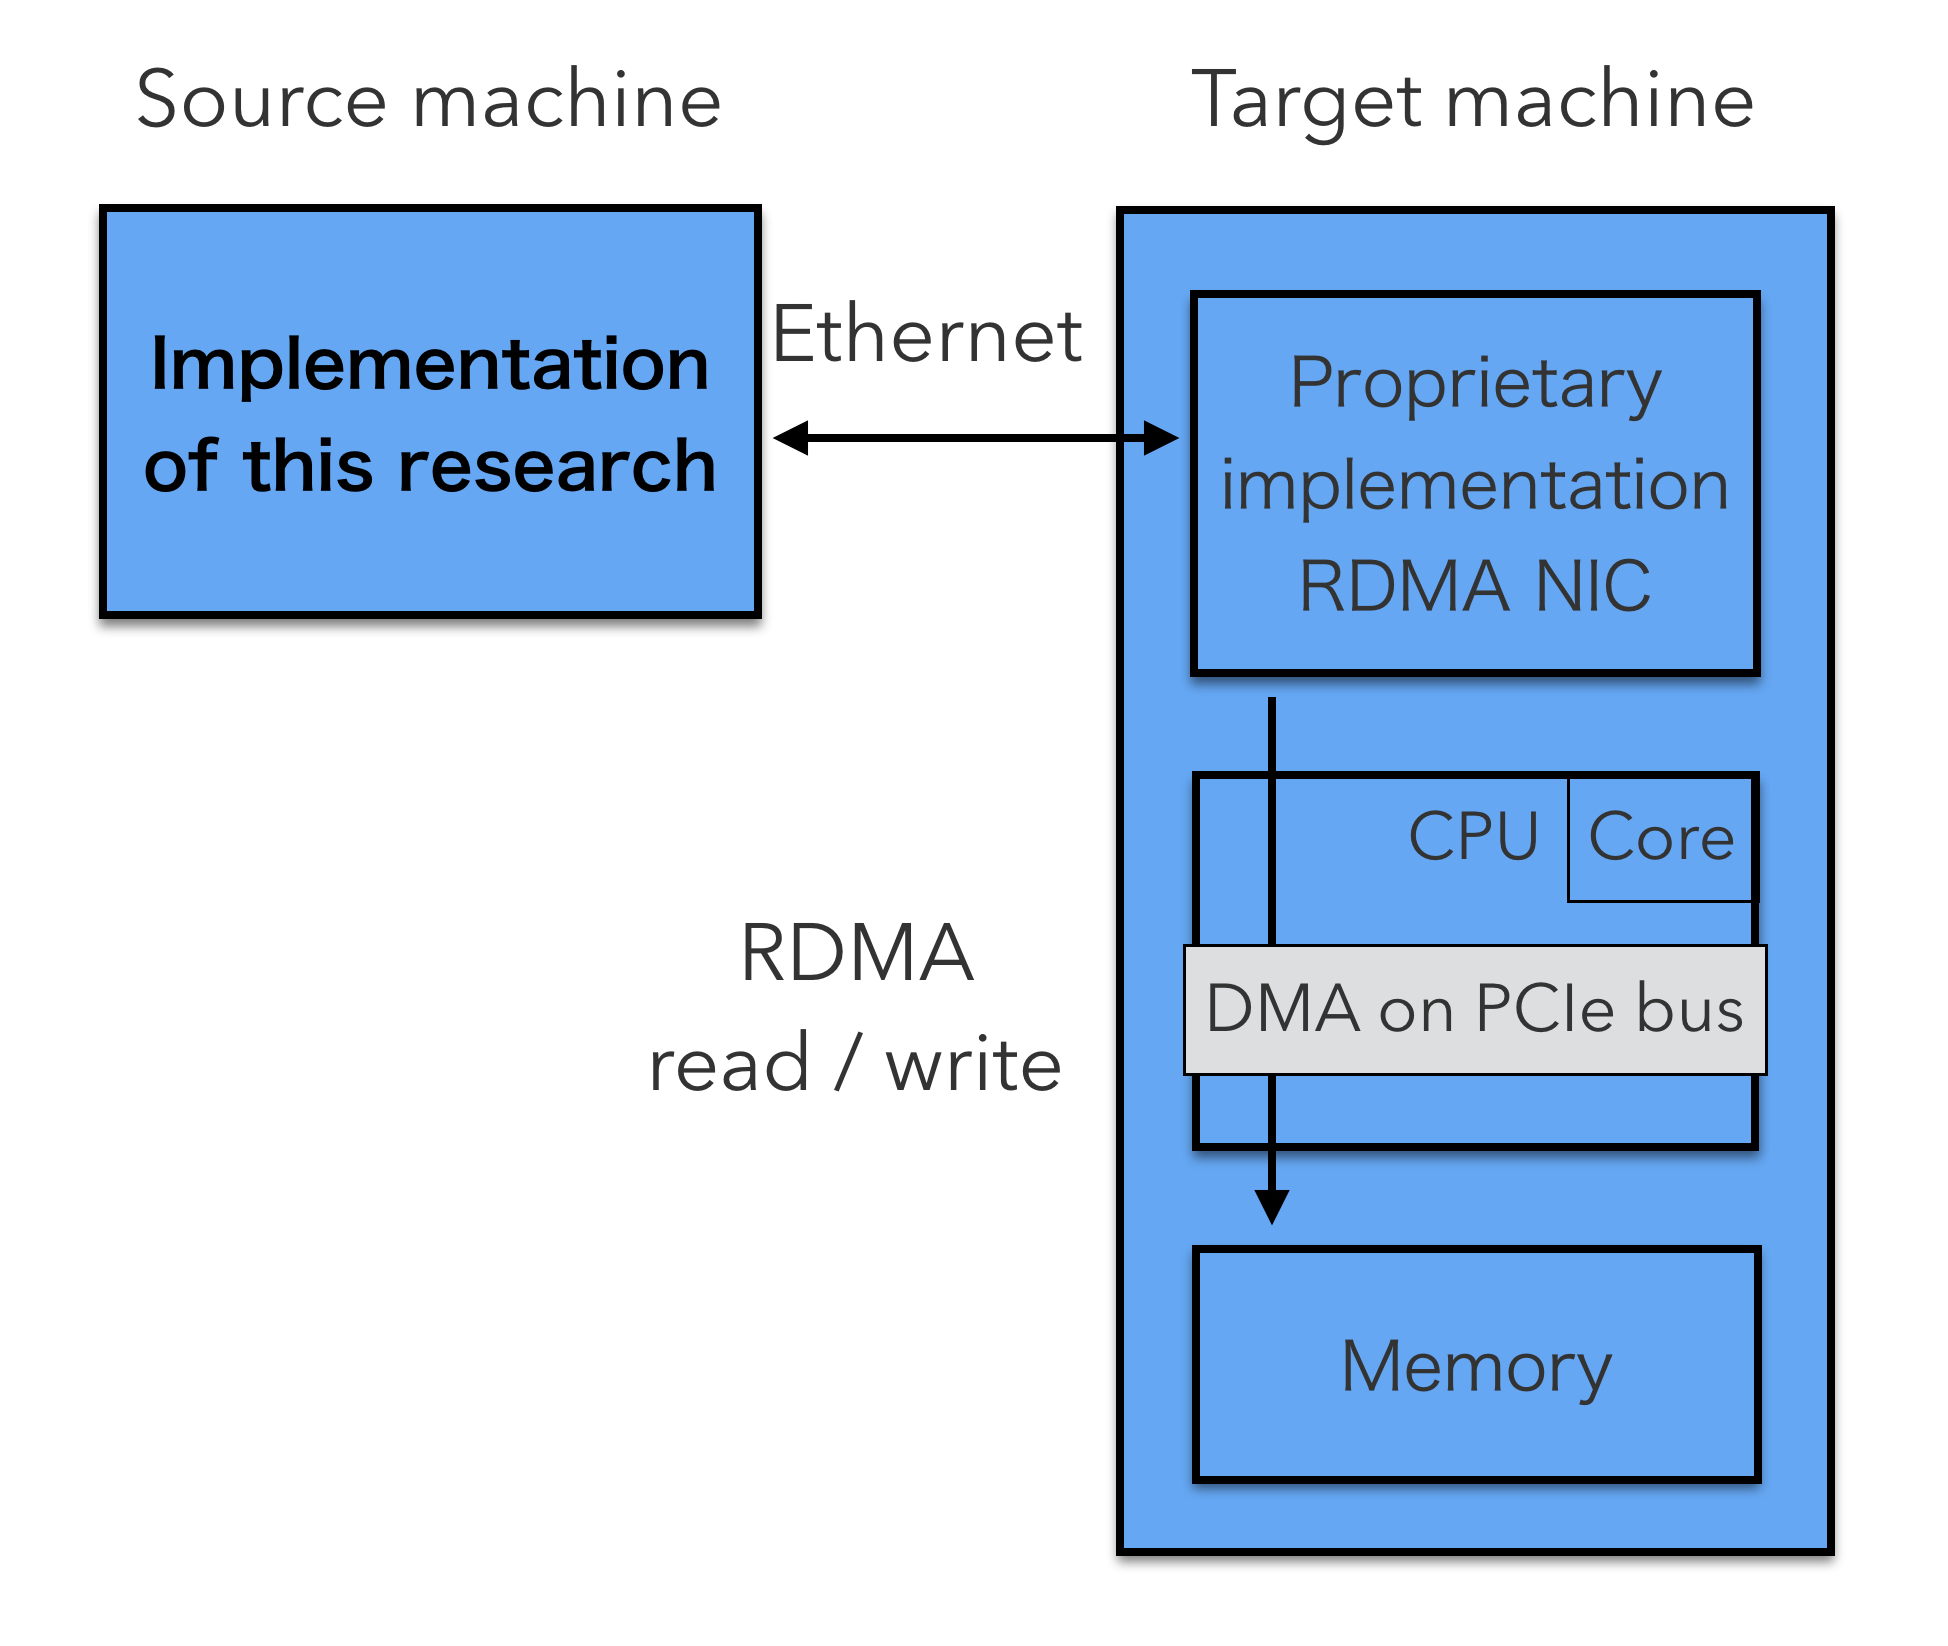
\includegraphics[bb=0 0 1000 800,width=15cm]{img/zentai.png}
    \end{center}
\end{figure}

\section{実装の前提情報}

本研究では,\ref{chap:approach}章で述べたように,
動作中のコンピュータのメインメモリの値を読むことによって監視対象ホストにおけるオペレーティングシステムのコンテキストを復元することを目的としている.
その手法として,RDMA NICを物理的に設置することで,この目的を達成することを試みている.

そこで,本研究の実装側のホストに与える情報を少なくすることが必要となる.
本セクションでは,本研究の実験において,実装したプログラムを実行するホストが持っている情報と,初期段階では持っていないが解析の結果導き出す情報を分類する.

\ref{chap:approach}章で述べたように,オペレーティングシステムのコンテキストの復元,
その中でもLinuxにおいてプロセス情報の一覧を出すために必要な情報は以下の三点である.

一点目は,init\_taskという,pidが0のプロセスのtask\_struct構造体の開始アドレスである.
init\_taskはコンピュータが起動する際に最初に実行されるプロセスであり,全てのプロセスは親プロセスを辿っていくことで,このプロセスにたどり着くことができる.
この情報は,実験に際して実装したプログラムを実行するホストは,知らないこととする.(いいのか?)

二点目は,task\_struct構造体の各フィールドの有無である.
Linuxカーネルでは,ビルドする際に,数千に及ぶ設定を記述し,マクロとして設定される.
この設定,kconfigによってtask\_structは,どのフィールドを有効にするか,マクロとして定義された構造体の実体は何になるのか,などが決まる.
kconfigの結果によって,フィールドが存在するか否か,またそのフィールドが先頭アドレスからどのくらいのオフセットを持った状態で保持されているかが決まる.
すなわち,kconfigの情報によって,task\_structのサイズや各フィールドの先頭アドレスからのオフセットが確定する.
このkconfigに関する情報は実験に際して実装したプログラムを実行するホストは知らないこととする.

三点目は,Linuxカーネルのバージョンに関する情報である.
本研究では,実験する際に,監視対象ホストのカーネルのバージョンと同じソースコードを使用した上で実験を行う.
当然,Linuxカーネルのバージョンに関する情報は知っている必要がある.
Linuxカーネルのバージョンは,実装ホストは持っている情報とする.
\ref{section:want}節で述べたもののうち,Linuxカーネルのバージョンは通知することとする

\section{実装の全体}

% ダンプしてくるということを書く.物理アドレスのマッピングに関しても書く

実験における第一段階として,\ref{section:want}節で述べたように,監視対象ホストのカーネルコンフィグおよびinit\_taskの先頭アドレスの仮想アドレスを知ることを目指す.
そこで,本研究では,この情報をメモリ上から探す.\ref{section:mem_dump}節で述べる実装では,取得できるメモリダンプを全て取得し,解析する手法に関して述べる.

第二段階として,与えられたLinuxカーネルのバージョンのソースコードより,カーネルコンフィグの一覧を抽出し,その文字列を取得したメモリダンプから文字列探索をする.
文字列探索の結果取得したカーネルコンフィグの値をパースし,メモリ上から監視対象ホストのカーネルコンフィグを復元する.
\ref{section:restore_kconfig}節で述べる実装では,カーネルコンフィグを復元する際の実装の詳細に関して記述する.

第三段階として,収集したカーネルコンフィグを元に手元のコンピュータでLinuxカーネルのソースコードに対してプリプロセスの処理を行い,task\_struct型を確定する.
また,\ref{section:approach}節で述べた,監視対象ホストで動いているプロセスの一覧情報を取得するための
さらに,ソースコード上にある\verb|__phys_addr|関数の実体を収集する.

最後に,この工程で得られた情報をもとに,libtlpで提唱されている手法を用いて,プロセスの一覧を正しく取得できることを確認する.

\section{mem\_dump.c}
\label{section:mem_dump}

第一の工程として,メモリの全ての情報を取得する.ソースコードは以下である.この実装を実装ホストで実行し,出力結果をファイルに格納する.
この実装では,libtlpを通して,監視対象ホストのメモリを全探索する.この実装の実行には長い時間(何分?)かかるため,アトミックな情報ではない.
そのため,ここで取得したメモリダンプは,解析には使えない.
ここで取得したメモリダンプは,System.mapのうち,init\_taskが配置されている仮想アドレス空間に関する情報および,Linuxカーネル 4.15.0におけるカーネルコンフィグに関する情報を収集するためのものである.

% Linuxカーネルにおける\verb|__phys_addr|関数,task\_struct型を決定するためのカーネルコンフィグに関する情報を収集することは\ref{chap:related_works}章で述べた.

\begin{itembox}[l]{実行方法}
    \begin{verbatim}
./dump_mem > dump
    \end{verbatim}
\end{itembox}

\begin{itembox}[l]{mem_dump.c}
    \begin{verbatim}
        ここにソースを貼り付ける.
    \end{verbatim}
\end{itembox}

\section{カーネルコンフィグの復元}
\label{section:restore_kconfig}

Linuxカーネル4.15.0におけるカーネルコンフィグの一覧は,下に示す通りである(あとではるかも)

これらのコンフィグに関する情報を以下のスクリプトで読み出す.

カーネルコンフィグには,各設定項目に対する値として,y,mや文字列,数値などがあり,設定しない項目については,その行がコメント行になるのに加えて,\verb|is not set|という文言が付け足される.
これらの特徴を踏まえ,本研究では,restore_kconfig.pyというスクリプトをPythonを用いて実装した.
このスクリプトでは,得られたメモリダンプから,stringsコマンドを用いて文字列を抽出し,そこからkconfigの特徴である,CONFIGという文字列を含む行をgrepコマンドを用いて抽出する.
実行するシェルスクリプトは以下である.

\begin{itembox}[l]{strings}
    \begin{verbatim}
strings dump | grep CONFIG > str_list
    \end{verbatim}
\end{itembox}

生成されたファイルに対して,上述したスクリプトを実行し,ファイルに書き出す.ここでは書き出すファイル名をrestored\_kconfigとする.

\begin{itembox}[l]{exec restore_kconfig.py}
    \begin{verbatim}
python restore_kconfig.py str_list > restored_kconfig
    \end{verbatim}
\end{itembox}

\begin{itembox}[l]{search config script}
    \begin{verbatim}
import sys

configs = [
    "CONFIG_64BIT", "CONFIG_X86_64", "CONFIG_X86",
    "CONFIG_INSTRUCTION_DECODER", "CONFIG_OUTPUT_FORMAT",
    "CONFIG_ARCH_DEFCONFIG", "CONFIG_LOCKDEP_SUPPORT",
    # 省略
    "CONFIG_ARCH_HAS_PMEM_API", "CONFIG_ARCH_HAS_UACCESS_FLUSHCACHE",
    "CONFIG_SBITMAP", "CONFIG_PARMAN", "CONFIG_STRING_SELFTEST"
]

# 有効な文字列が見つかった場合は1を返す
def classification(l, s):

    if "#if" in l or "#endif" in l:
        # sys.stderr.write("No!! -> Macro, "+l)
        return 0

    if l[:3] != "CON" and l[:3] != "# C":
        # sys.stderr.write("No!! -> NOT CONFIG, "+l)
        return 0

    if s + "=y" in l:
        print(s + "=y")
        return 1
    elif s + "=m" in l:
        print(s + "=m")
        return 1
    elif s + " is not set" in l:
        print("# " + s + " is not set")
        return 1
    elif s + '=' in l:
        print(l)
        return 1
    else:
        # sys.stderr.write("No!! -> No match, "+l)
        return 0

    \end{verbatim}
\end{itembox}

\begin{itembox}[l]{search config script2}
    \begin{verbatim}
def search_config_str(file_name, s):
    ld = open(file_name)
    lines = ld.readlines()
    ld.close()

    for line in lines:
        if line.find(s) >= 0:
            if classification(line[:-1], s):
                return 1
    return 0


def search(file_name):
    for s in configs:
        # print("Searching "+s+" .....")
        if not search_config_str(file_name, s):
            # print("# Cannot find " + s)
            sys.stderr.write("# Cannot find " + s)


def usage():
    print("usage: python find_kconfig.py path/to/str_list")


def main():
    args = sys.argv
    if len(args) < 2:
        usage()
        return 0

    file_name = args[1]
    search(file_name)


if __name__ == "__main__":
    main()

    \end{verbatim}
\end{itembox}

上述した処理によって得られたrestored_kconfigというファイルを,後述するビルド時にコンフィグとして利用する.

\section{Linuxカーネルをプリプロセッサに通す}
\label{section:preprocess}

この工程では,収集したカーネルコンフィグを元に手元のコンピュータでLinuxカーネルのソースコードに対してプリプロセスの処理を行い,task\_struct型,
および\verb|__phys_addr|関数など,\verb|process-list.c|の影響のあるソースコードを確定する.

また,pid 0のプロセスのtask\_struct構造体の先頭アドレスを知るため,またそれぞれのフィールドの先頭アドレスからのオフセットを確定させるため,オフセットを得る処理を施す.

まずは,事前に知らされた情報であるLinuxカーネルのバージョンより,適合したカーネルを取得する.
このソースコードに対して,\ref{section:restore_kconfig}節で生成したファイルをコンフィグとして埋め込む.

\begin{itembox}[l]{build Linux kernel}
    \begin{verbatim}
        cd /path/to/linux-source-4.15.0
        cp /path/to/restored_kconfig .config
    \end{verbatim}
\end{itembox}

また,この工程では,カーネルビルド時におけるtask\_struct型をバイナリではなくテキストファイルとして取得する必要があるため,
マクロを適用した直後の状態,すなわちプリプロセッサに通した直後の状態を保存するため,ビルド時の設定に変更を加える.
Linuxカーネルにおいては,ビルド時にMakefileを使用するため,このファイルを編集する.
例として,Linuxカーネル,バージョン4.15.0-74-genericにおいては,Makefileの447行目付近に,\verb|-save-temps|オプションを以下のような形で設定する.

\begin{itembox}[l]{-save-tempsオプションの設定・変更前}
    \begin{verbatim}
KBUILD_AFLAGS   := -D__ASSEMBLY__
KBUILD_CFLAGS   := -Wall -Wundef -Wstrict-prototypes -Wno-trigraphs \
        -fno-strict-aliasing -fno-common -fshort-wchar \
        -Werror-implicit-function-declaration \
        -Wno-format-security \
        -std=gnu89
KBUILD_CPPFLAGS := -D__KERNEL__
KBUILD_AFLAGS_KERNEL :=
KBUILD_CFLAGS_KERNEL :=
KBUILD_AFLAGS_MODULE  := -DMODULE
KBUILD_CFLAGS_MODULE  := -DMODULE
KBUILD_LDFLAGS_MODULE := -T $(srctree)/scripts/module-common.lds
    \end{verbatim}
\end{itembox}

\begin{itembox}[l]{-save-tempsオプションの設定・変更後}
    \begin{verbatim}
KBUILD_AFLAGS   := -D__ASSEMBLY__
KBUILD_CFLAGS   := -Wall -Wundef -Wstrict-prototypes -Wno-trigraphs \
        -fno-strict-aliasing -fno-common -fshort-wchar \
        -Werror-implicit-function-declaration \
        -Wno-format-security \
        -std=gnu89

KBUILD_CFLAGS += -save-temps=obj

KBUILD_CPPFLAGS := -D__KERNEL__
KBUILD_AFLAGS_KERNEL :=
KBUILD_CFLAGS_KERNEL :=
KBUILD_AFLAGS_MODULE  := -DMODULE
KBUILD_CFLAGS_MODULE  := -DMODULE
KBUILD_LDFLAGS_MODULE := -T $(srctree)/scripts/module-common.lds
    \end{verbatim}
\end{itembox}

設定ファイルを書き終わったらビルドを行う.

\begin{itembox}[l]{ビルド}
    \begin{verbatim}
make -j10
    \end{verbatim}
\end{itembox}

\section{task\_struct構造体の確定}
\label{section:define_task_struct}

本セクションでは,\ref{section:preprocess}節で述べた工程を経た結果生成された中間ファイルから,task\_struct構造体を導出し,プロセス情報一覧の表示に必要なフィールドのオフセットを求める.

Linuxカーネルのビルドが完了すると,上述したMakefileのKBUILD_CFLAGSの設定によって,中間ファイルを含む巨大なディレクトリおよび,vmlinux,bzImageが作成される.
本研究では,このビルドされたbzImageは使用しない.

ビルドの際に,プリプロセッサの出力を残したことで,ソースコード中の全てのマクロおよびincludeされたファイルが展開された状態のソースコードがファイルとして残っている.
例として/kernel/pid.cをあげると,このファイルでは,task\_struct構造体を呼び出している箇所があるが,このファイルをプリプロセッサに通すことで,pid.iが作成される.
pid.iを通して見てみると,task\_struct構造体が全て展開され,そこから参照される全ての構造体やtypedefの情報がソースコード上にあることがわかる.

この中間ファイルから,task\_structおよびそこから参照される全ての要素を抽出し,以下のソースコードの\verb|struct task_struct{};|と書かれている部分に記述する.
このファイルをビルドすることで,task\_struct構造体の各フィールドのオフセットを導出する.

\begin{itembox}[l]{print_offset.cの雛形}
    \begin{verbatim}
#include <stdio.h>
#include <stddef.h>
#include <unistd.h>

struct task_struct{};

int main()
{
    size_t size = sizeof(struct task_struct);
    printf("task_struct size: %lu\n\n", size);
    size_t offset;
    offset = offsetof(struct task_struct, state);
    printf("state: %zu\n", offset);
    offset = offsetof(struct task_struct, pid);
    printf("pid: %zu\n", offset);
    offset = offsetof(struct task_struct, children);
    printf("children: %zu\n", offset);
    offset = offsetof(struct task_struct, sibling);
    printf("sibling: %zu\n", offset);
    offset = offsetof(struct task_struct, comm);
    printf("comm: %zu\n", offset);
    offset = offsetof(struct task_struct, real_parent);
    printf("real_parent: %zu\n", offset);
    return 0;
}
    \end{verbatim}
\end{itembox}

print\_offset.cの実行結果は以下の通りである.

\begin{itembox}[l]{./print_offset}
    \begin{verbatim}
$ ./print_offset
# task_struct size: 9088

# state: 16
# pid: 2216
# children: 2248
# sibling: 2264
# comm: 2640
# real_parent: 2232
    \end{verbatim}
\end{itembox}

ここで得られたオフセットを用いて,後述する\ref{subsection:find_init_task}節にてinit\_taskの開始アドレスを求める.

\subsection{init\_taskの開始アドレスの算出}
\label{subsection:find_init_task}

本セクションでは,プロセスIDとして0を持つプロセスである,init\_taskの先頭開始アドレスの算出開始アドレスの算出アドレスを算出する.

init\_taskの開始アドレスは,監視対象ホストの,/proc/kallsymsに記述されているが,その開始アドレスは本研究の実験環境においては,
実装したプログラムを実行するホストは情報として持っていない.そのため,後述する手法を用いてその開始アドレスを算出する.

\ref{section:mem_dump}節では,ネットワーク越しに,監視対象ホストのメモリダンプを取得する工程について記述した.
このメモリダンプからプロセスID 0をもつinit\_taskを探す.
init\_taskはtask\_struct構造体であるため,メモリダンプの中から,init\_taskに特有の文字列をなどを探し,それを目印としてinit\_taskの先頭アドレスを算出する.

本研究においては,task\_struct構造体の,commフィールドの値に着目した.
commフィールドには,プロセスに関する情報のうち,実行可能ファイルの名前が16Byteで記載されている.
init\_taskにおけるcommフィールドの値は,swapper/0であるため,この値をメモリダンプから,以下のスクリプトを用いて検索を行う.

\begin{itembox}[l]{find swapper/0}
    \begin{verbatim}
xxd dump | grep swapper/0
    \end{verbatim}
\end{itembox}

この値から,\ref{section:define_task_struct}節にて求めた,commフィールドの値を引き,
そこからさらに,ブートローダの使用領域である128KBを足すことで,init\_taskの先頭アドレスを算出する.

% 131072 = 128KB!!
% 128KBはBIOSの領域?
% (xxd dump | grep swapper/0のアドレス) - commのoffset + 128KBがinit_taskの先頭アドレス.

% KASLRを自然と回避することになる.多分

\section{プロセス一覧の表示}
\label{subsection:process-list}

% \ref{section:preprocess}で得ることができたソースをもとに,process-listを改造したものに関する説明をここに書く(もう動いてはいるので,整理して書く.)

以上の実装により得られた値を用いて,\ref{subsection:upa_process}節で述べたprocess-list.cのうち,
監視対象ホストの環境に依存した部分を書き換えることで,プロセスの一覧を取得する.

\subsection{環境に依存するパラメータ}

本セクションでは,プロセスの一覧を得る上で,マシンごとに異なる設定を述べる.

一点目として,カーネル空間に仮想アドレスにおける仮想アドレスから物理アドレスへ変換する際に使用する関数の実体が異なる.
/proc/kallsymsに書いてある値をはじめとして,子プロセスの開始アドレスを格納しているフィールドには,カーネル空間における仮想アドレスが格納されているが,
本研究においてメモリアドレスを指定する際には,物理アドレスを指定する必要がある.
Linuxカーネル4.15.0においては,変換に用いる関数およびその中で使用されているシンボルは,
CONFIG_DEBUG_VIRTUALという設定や,64bitかどうかを示す値であり,この値はソースコードからマクロを辿っていくことで知ることが可能である.
本研究では,\ref{section:restore_kconfig}節にて述べたように,復元したマクロの値を参照しつつ,この関数の実体を確定させる.

二点目として,監視対象ホストの上におけるtask\_struct構造体におけるオフセットの値である.
この値に関しては,\ref{section:define_task_struct}節で求めたため,その値を以下の6行に記載する.

\begin{itembox}[l]{macros}
    \begin{verbatim}
#define OFFSET_HEAD_STATE 16
#define OFFSET_HEAD_PID 2216
#define OFFSET_HEAD_CHILDREN 2248
#define OFFSET_HEAD_SIBLING 2264
#define OFFSET_HEAD_COMM 2640
#define OFFSET_HEAD_REAL_PARENT 2232
    \end{verbatim}
\end{itembox}

\section{実装のまとめ}

% この章は,相当長くなるので,まとめを書く.

本章では,監視対象ホストに関する情報として,動作しているLinuxカーネルのバージョンのみを実装したプログラムを実行するホストに与えた.
その上で,RDMAのNetTLP実装を用いてメモリダンプを取得し解析を行うことで,
カーネルコンフィグをはじめとした,プロセス一覧の取得に必要な情報を収集するための実装について述べた.
